Before we do any coding, we must learn the theory behind how computer systems work, which all starts from memory management and CPU architecture. We will use C with the gcc compiler, along with MIPS and NASM assembler. It is imperative to learn these two since given that you know a high level language pretty well (Python in my case), you want to learn C to appreciate the things Python does for you, and you want to learn Assembly to appreciate the things C does for you.\footnote{https://www.youtube.com/watch?v=XlvfHOrF26M}. 

To start off, we want a big overall picture of high a computer works. We introduce this with the simplest model of the computer, the Von Nuemann architecture. It consists of a \textbf{central processing unit} (CPU), \textbf{memory}, and an \textbf{input/output} (I/O) system. We show a diagram of this first for conciseness in Figure \ref{fig:von_neumann_arch}. 

\begin{figure}[H]
  \centering 
  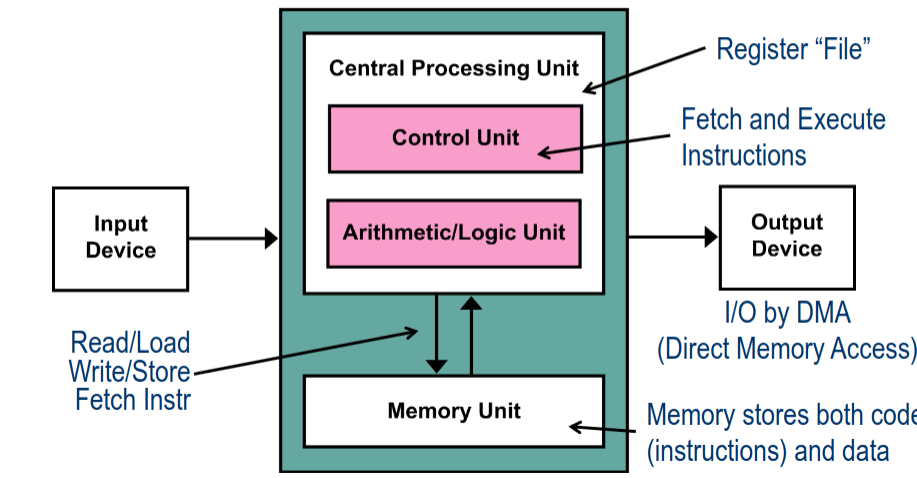
\includegraphics[scale=0.4]{img/von_neumann_arch.png}
  \caption{von Neumann Architecture} 
  \label{fig:von_neumann_arch}
\end{figure}

We will go through these one by one, touching on C and Assembly along the way, but the implementation of these things can differ by the \textbf{computer architecture}, so let's list some of the basic ones. 

\begin{definition}[Computer Architecture]
  The \textbf{computer architecture} is the design of the computer, which includes the CPU, memory, and I/O system. There are many different architectures, but we will focus on the most common ones.
\end{definition}

We first go over some basic theoretical properties of basic data types, focusing on C, and then we cover all the stuff about memory and then all the stuff about the CPU. This is a natural progression since to work with data, you must first know where to store the data and how it is stored (the memory), and then you want to know how data is manipulated (the CPU). 

